% =====================================================================
% =====================================================================
\section{\texorpdfstring{Selection and analysis of word format}{Selection of word format}}\label{sec:resultados-formato}

This section presents the results of the validation of the 10 formats (Section~\ref{subsec:validacao}). The results are grouped by the number of the configuration, which sets $M$, $C$ and the size of the inversion circuit (Section~\ref{subsec:configuracoes-bs}): group 1 ($M = 128$, $C = 8$, $16 \times 16$ circuit), group 2 ($M = 256$, $C = 8$, $32 \times 32$ circuit) and group 3 ($M = 256$, $C = 16$, $16 \times 16$ circuit). All configurations of a group use the same circuit, and only the modulation, $K$ and IoTh change between them.

For each group, the section presents the effect of the format on the SNR increase, the chosen formats, and how much of the increase over LMMSE comes from decentralization and how much from the format. Then, Section~\ref{subsec:perfis-mobilidade} shows whether the choice of format changes with the mobility profile. \textcolor{red}{Depois, a Seção~\ref{sec:resultados-curvas} mostra as curvas de SER dos três grupos.} The hardware, throughput and delay results are presented by test condition, because each condition has its own architecture, set by its cycle limit (Section~\ref{sec:resultados-hardware}).

% ---------------------------------------------------------------------
\subsection{\texorpdfstring{\textcolor{red}{Grupo 1: $M = 128$, $C = 8$}}{Grupo 1: M = 128, C = 8}}\label{subsec:resultados-grupo1}\label{subsec:mapas-perda}
% ---------------------------------------------------------------------


\begin{figure}[!htb]
\caption{\textcolor{red}{Maior aumento de SNR, em dB, no grupo 1, configurações 1A a 1H ($M = 128$, $C = 8$, $M_c = 16$).}}
\label{fig:mapa-grupo1}
\vspace{4pt} % a classe zera o espaço entre a caption e a figura
\centering
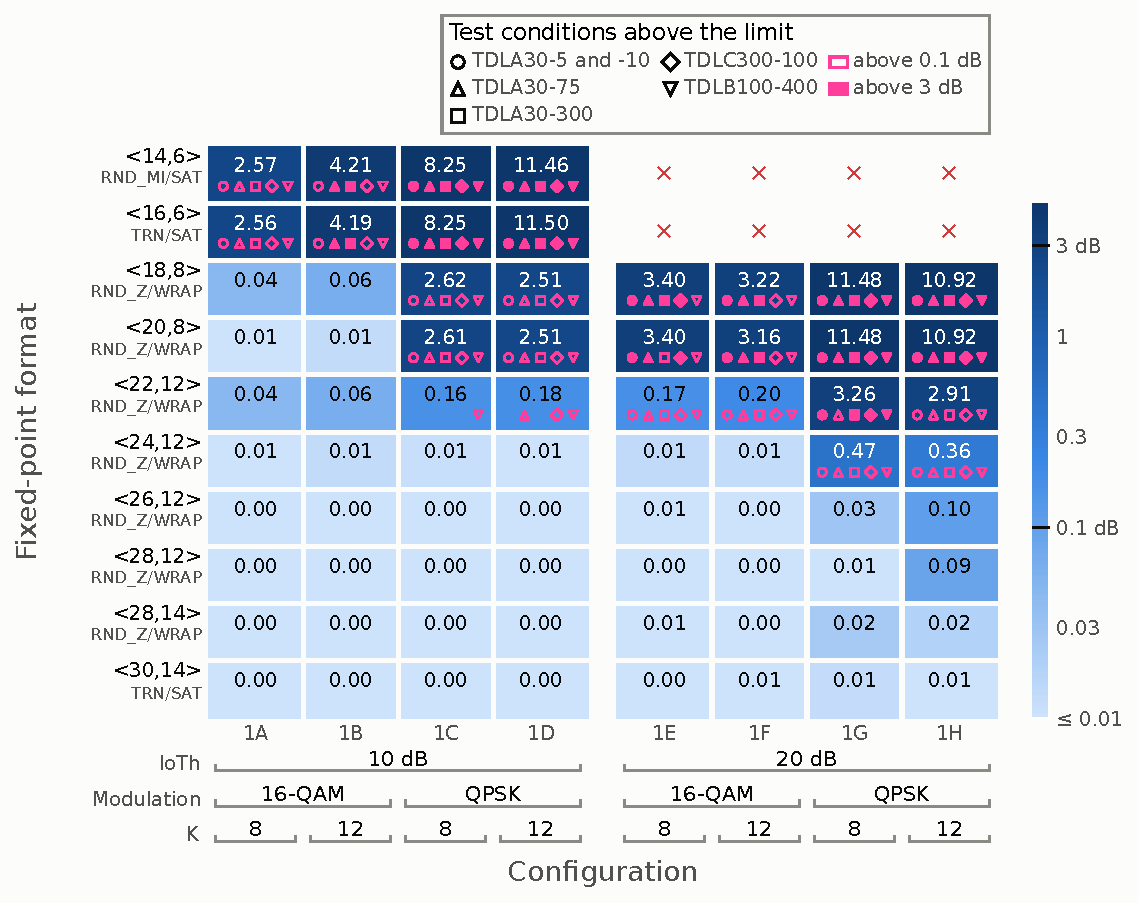
\includegraphics[width=\textwidth]{Images/RESULTADOS/mapa_snr_grupo1.pdf}
\vspace{4pt}
\legend{\textcolor{red}{Fonte: a autora. Abaixo do formato, o modo de quantização e o de estouro, sem o prefixo AP\_.}}
\end{figure}

Figure~\ref{fig:mapa-grupo1} shows, on a logarithmic color scale, the largest SNR increase of each format (rows) in each configuration (columns), among the 5 simulated test conditions (Section~\ref{subsec:setup_condicoes}). Below the value, unfilled symbols mark the test conditions above 0.1~dB, and filled symbols, those above 3~dB. The circle stands for TDLA30-5 and TDLA30-10, which share the same SER curves. A $\times$ marks a cell where some test condition does not reach $\mathrm{SER} = 10^{-2}$. The maps of groups 2 and 3 follow the same layout.

For each threshold, the chosen format is the smallest one in which all configurations stay within it (Section~\ref{sec:formato}): $\langle 24,12\rangle$ for 3~dB and $\langle 26,12\rangle$ for 0.1~dB. The QPSK configurations with IoTh of 20~dB (1G and 1H) set both formats. When only the configurations with IoTh of 10~dB (1A to 1D) are considered, the chosen formats are $\langle 18,8\rangle$ and $\langle 24,12\rangle$, respectively.


% -----------------------

\label{sec:resultados-descentralizacao}\label{subsec:descentralizacao}%

\begin{figure}[!htb]
\caption{\textcolor{red}{Aumento de SNR do BCD-MMSE sobre o LMMSE no grupo 1 ($M = 128$, $C = 8$, $M_c = 16$), no pior caso de cada barra.}}
\label{fig:descentralizacao-grupo1}
\vspace{4pt} % a classe zera o espaço entre a caption e a figura
\centering
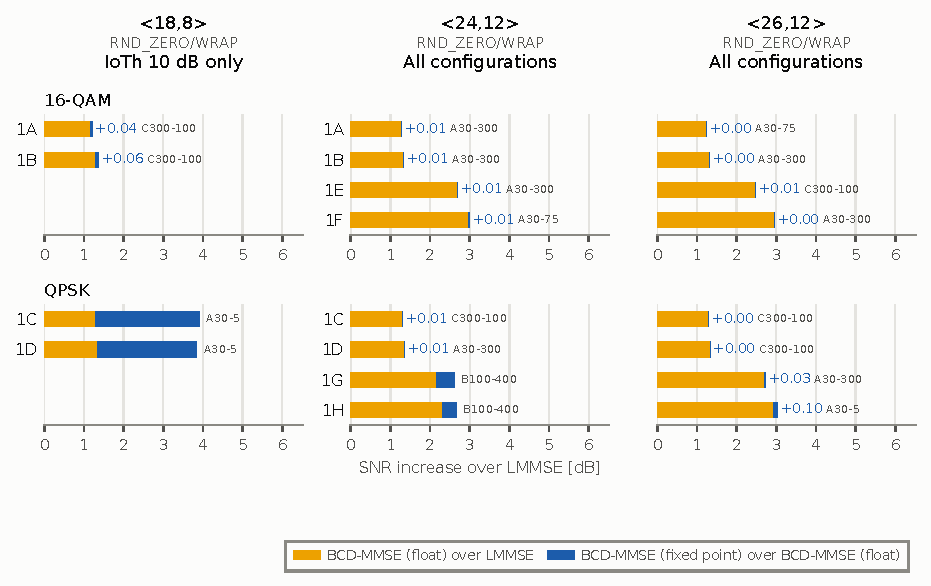
\includegraphics[width=\textwidth]{Images/RESULTADOS/descentralizacao_grupo1.pdf}
\vspace{4pt}
\legend{\textcolor{red}{Fonte: a autora.}}
\end{figure}

Figure~\ref{fig:descentralizacao-grupo1} illustrates the source of the SNR gain provided by BCD-MMSE over LMMSE at an $\mathrm{SER}$ of $10^{-2}$. The yellow bar represents the gain resulting from decentralization, that is, the difference between LMMSE and floating-point BCD-MMSE. The blue bar represents the gain (or impact) attributed to the numerical format, that is, the difference between floating-point and fixed-point BCD-MMSE, with the specific value indicated at the end of the bar. Each plot corresponds to a chosen format from the group (Table~\ref{tab:formatos-escolhidos}), and each bar represents a specific configuration. For each configuration, the test condition under which the format yields the greatest SNR increase was selected, and the name of this condition is labeled next to the bar.

In Group 1, decentralization provides the largest SNR gain when the IoTh is 20~dB. With 16-QAM, the gain attributed to the numerical format is negligible. In contrast, with QPSK, this gain is significantly larger, reaching 2.6~dB for the $\langle 18,8\rangle$ format, which exceeds the gain provided by decentralization. Thus, QPSK appears to be more sensitive to the approximations introduced by the numerical format than 16-QAM.

% -----------------------

\FloatBarrier
% ---------------------------------------------------------------------
\subsection{\texorpdfstring{\textcolor{red}{Grupo 2: $M = 256$, $C = 8$}}{Grupo 2: M = 256, C = 8}}\label{subsec:resultados-grupo2}\label{subsubsec:mapa-grupo2}
% ---------------------------------------------------------------------

\begin{figure}[!htb]
\caption{\textcolor{red}{Maior aumento de SNR, em dB, no grupo 2, configurações 2A a 2H ($M = 256$, $C = 8$, $M_c = 32$).}}
\label{fig:mapa-grupo2}
\vspace{4pt} % a classe zera o espaço entre a caption e a figura
\centering
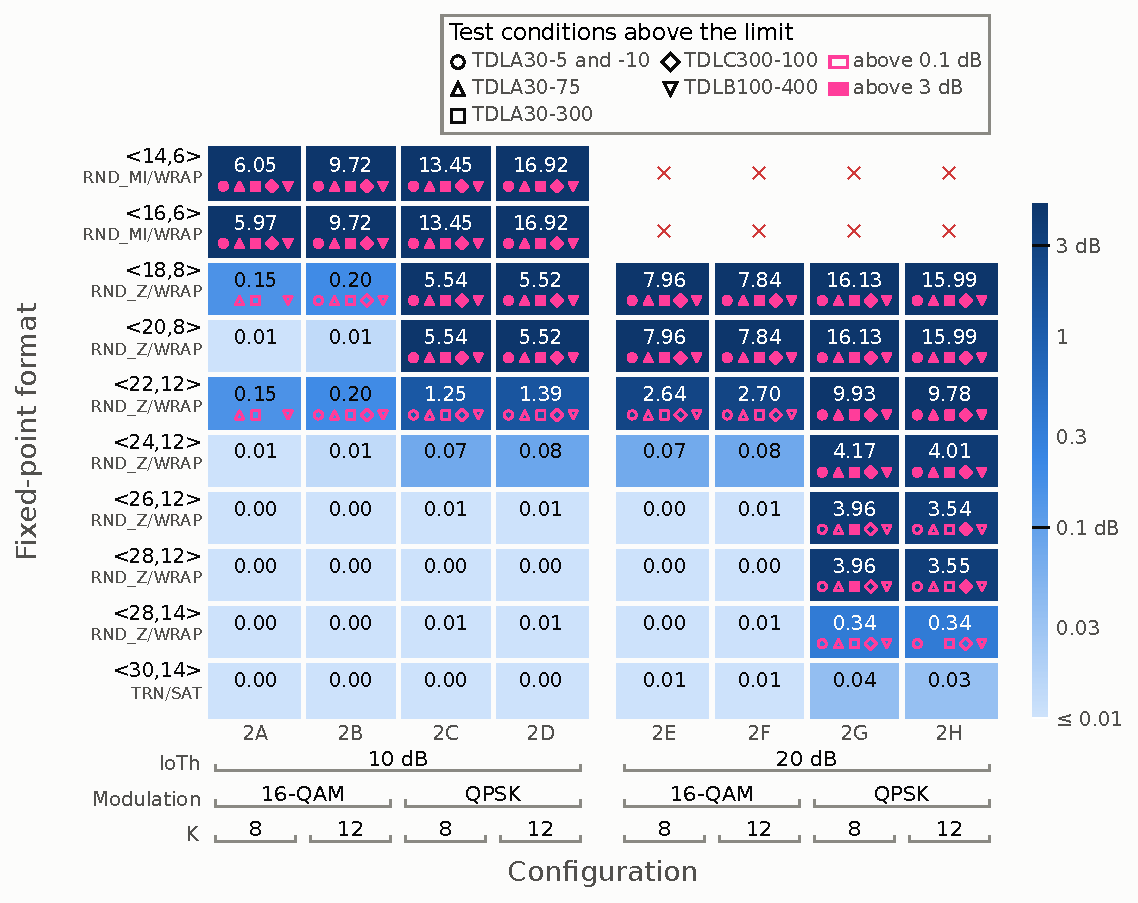
\includegraphics[width=\textwidth]{Images/RESULTADOS/mapa_snr_grupo2.pdf}
\vspace{4pt}
\legend{\textcolor{red}{Fonte: a autora. Abaixo do formato, o modo de quantização e o de estouro, sem o prefixo AP\_.}}
\end{figure}

\begin{figure}[!htb]
\caption{\textcolor{red}{Aumento de SNR do BCD-MMSE sobre o LMMSE no grupo 2 ($M = 256$, $C = 8$, $M_c = 32$), no pior caso de cada barra.}}
\label{fig:descentralizacao-grupo2}
\vspace{4pt} % a classe zera o espaço entre a caption e a figura
\centering
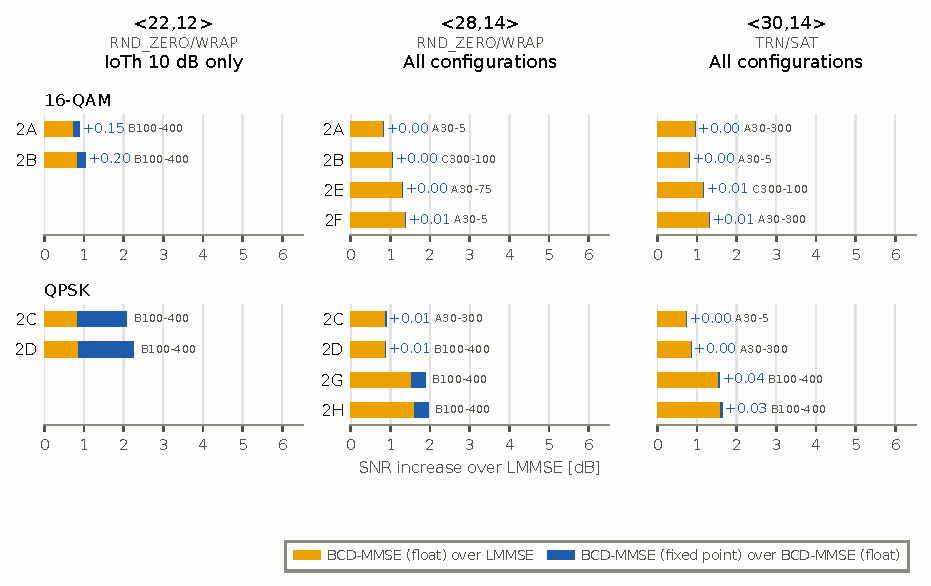
\includegraphics[width=\textwidth]{Images/RESULTADOS/descentralizacao_grupo2.pdf}
\vspace{4pt}
\legend{\textcolor{red}{Fonte: a autora.}}
\end{figure}

Group 2 has twice as many antennas as group 1, with the same number of clusters. Thus, each cluster has 32 antennas, not 16. In the map (Figure \ref{fig:mapa-grupo2}), the greatest increase in SNR in the smaller formats is greater than in group 1. Furthermore, the increase remains above 3 dB even in larger formats. In 2G and 2H, this goes up to $\langle 28,12\rangle$, while 1G and 1H remain below 3 dB from $\langle 24,12\rangle$. Therefore, the chosen formats are larger: $\langle 28,14\rangle$ at the 3 dB limit and $\langle 30,14\rangle$ at the 0.1 dB limit. As in group 1, the two are defined by 2G and 2H, with QPSK and IoTh of 20~dB.

In 2G and 2H, from $\langle 24,12\rangle$ to $\langle 28,12\rangle$, the increase hardly changes. These formats only gain fractional bits. The increase only decreases at $\langle 28,14\rangle$, which has 2 more integer bits. Therefore, group 2 needs more integer bits than group 1. A likely explanation is the SNR at which the group operates. With more antennas, the equalizers need less SNR, as also happens in \cite{zhao2025jsac}. In the simulation, the symbol energy $E_s$ is fixed, and the SNR varies according to the thermal noise power, $\sigma^2$ (Equation~\ref{eq:snr}). With a fixed IoTh, the interference scales with $\sigma^2$ (Equation~\ref{eq:iot}). Consequently, as the SNR decreases, the combined noise and interference become stronger, causing $\hat{\mathbf R}_{cc}$ to increase as well. Since $\mathbf G_c$ is formed by adding $\hat{\mathbf R}_{cc}$ to the channel term (Section~\ref{subsec:bcd}), the elements of $\mathbf G_c$ also increase. At the same SNR, an IoTh of 20 dB results in ten times more noise-plus-interference than an IoTh of 10 dB, leading to even larger values for these elements.
In Figure \ref{fig:descentralizacao-grupo2}, decentralization increases the SNR less than in group 1. That is, with more antennas, the BCD-MMSE gets closer to the LMMSE, as also happens in \cite{zhao2025jsac}. The increase in format size is also smaller because the chosen formats are larger. However, as in group 1, it is larger with QPSK than with 16-QAM.


% ---------------------------------------------------------------------
\subsection{\texorpdfstring{\textcolor{red}{Grupo 3: $M = 256$, $C = 16$}}{Grupo 3: M = 256, C = 16}}\label{subsec:resultados-grupo3}\label{subsubsec:mapa-grupo3}
% ---------------------------------------------------------------------

\begin{figure}[!htb]
\caption{\textcolor{red}{Maior aumento de SNR, em dB, no grupo 3, configurações 3A a 3H ($M = 256$, $C = 16$, $M_c = 16$).}}
\label{fig:mapa-grupo3}
\vspace{4pt} % a classe zera o espaço entre a caption e a figura
\centering
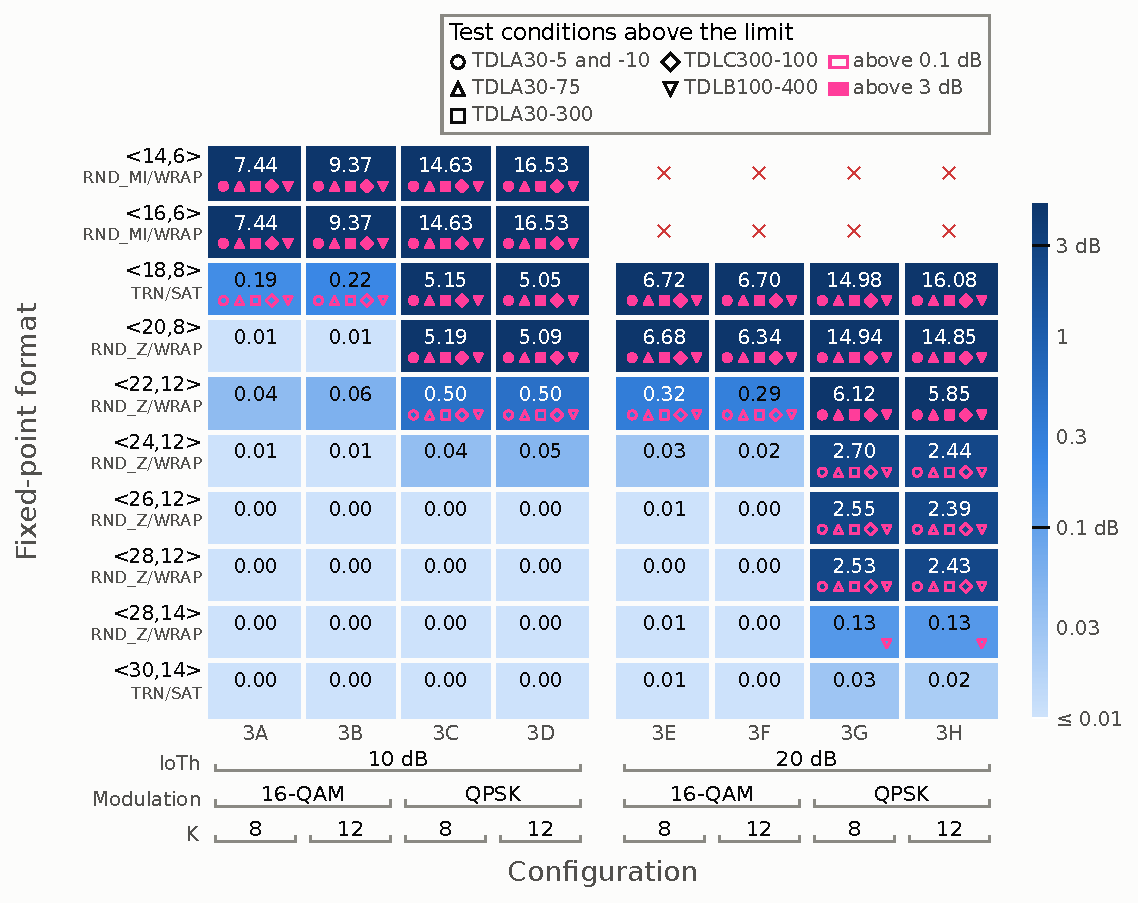
\includegraphics[width=\textwidth]{Images/RESULTADOS/mapa_snr_grupo3.pdf}
\vspace{4pt}
\legend{\textcolor{red}{Fonte: a autora. Abaixo do formato, o modo de quantização e o de estouro, sem o prefixo AP\_.}}
\end{figure}

\begin{figure}[!htb]
\caption{\textcolor{red}{Aumento de SNR do BCD-MMSE sobre o LMMSE no grupo 3 ($M = 256$, $C = 16$, $M_c = 16$), no pior caso de cada barra.}}
\label{fig:descentralizacao-grupo3}
\vspace{4pt} % a classe zera o espaço entre a caption e a figura
\centering
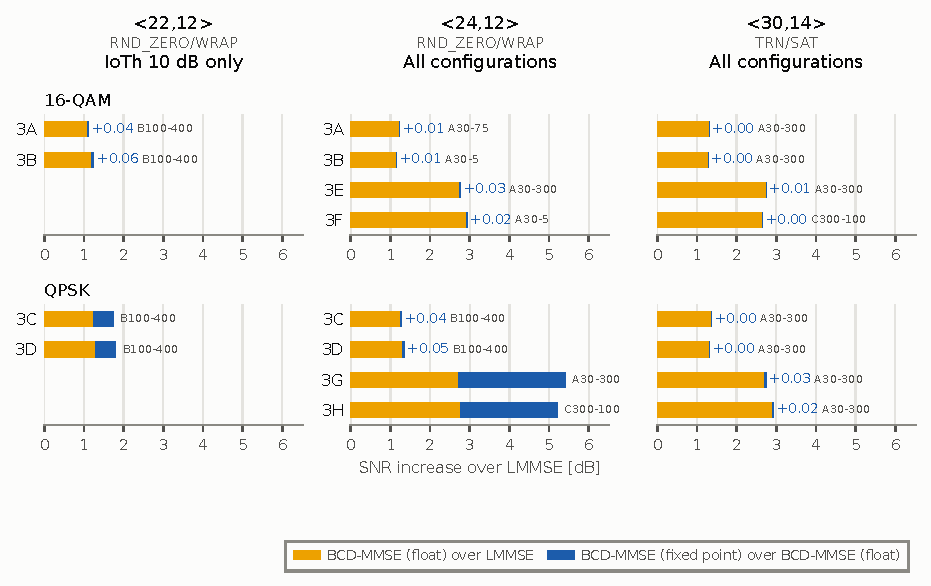
\includegraphics[width=\textwidth]{Images/RESULTADOS/descentralizacao_grupo3.pdf}
\vspace{4pt}
\legend{\textcolor{red}{Fonte: a autora.}}
\end{figure}


Group 3 has the same number of antennas as Group 2, but twice the number of clusters. Consequently, each cluster contains 16 antennas, just as in Group 1. As shown in the map (Figure~\ref{fig:mapa-grupo3}), the most significant gain for smaller formats occurs near Group 2. However, at the 3~dB threshold, the format is $\langle 24,12\rangle$, the same as in Group 1 and smaller than the $\langle 28,14\rangle$ format found in Group 2. This suggests that, in addition to the total number of antennas, the cluster size also influences the format.


For the $\langle 24,12\rangle$ format, 3G and 3H lie close to the 3~dB threshold. In subsequent formats, similar to what is observed in Group 2, the gain for these cases remains nearly constant up to $\langle 28,12\rangle$, only decreasing when two additional bits are introduced in the $\langle 28,14\rangle$ format. Even then, it remains above 0.1~dB. Therefore, at the 0.1~dB threshold, the format is $\langle 30,14\rangle$, which is the same as in Group 2.

\label{subsubsec:descentralizacao-grupo3}%

In Figure~\ref{fig:descentralizacao-grupo3}, decentralization yields a greater increase in SNR compared to Group 2, bringing it closer to the levels seen in Group 1. Since the clusters contain fewer antennas, each one utilizes a smaller block of the covariance matrix. With a higher number of clusters, the BCD-MMSE performance deviates further from the LMMSE, a phenomenon also noted in \cite{zhao2025jsac}. Using QPSK, for the $\langle 24,12\rangle$ format, the gain provided by the format for 3G and 3H is nearly equivalent to the gain achieved through decentralization. For $\langle 22,12\rangle$, with an IoTh of only 10~dB, the gap is smaller than in group 2.


Thus, across the three groups, the primary factor driving the divergence between BCD-MMSE and LMMSE depends on the modulation scheme. With 16-QAM, the impact of the numerical format is almost negligible, and the decentralization effect carries more weight. With QPSK, for the formats at the 3~dB threshold, the numerical format carries as much weight as the decentralization, or even more; this is the case for $\langle 18,8\rangle$ in group 1, $\langle 22,12\rangle$ in group 2, and $\langle 24,12\rangle$ in group 3. For the formats at the 0.1~dB threshold, the decentralization effect is the dominant factor in all cases.

\FloatBarrier
% ---------------------------------------------------------------------
\subsection{\texorpdfstring{\textcolor{red}{Formatos escolhidos}}{Formatos escolhidos}}\label{subsec:formatos-escolhidos}
% ---------------------------------------------------------------------
\begin{table}[htbp]
\caption{\textcolor{red}{Formatos escolhidos em cada grupo de configurações.}}
\label{tab:formatos-escolhidos}
\vspace{4pt} % a classe zera o espaço entre a caption e a tabela
\centering
\footnotesize
\renewcommand{\arraystretch}{1.2}
\setlength{\tabcolsep}{3pt}
\begin{tabular}{>{\raggedright\arraybackslash}p{2.4cm}ccc}
\toprule
\textbf{Criterion} & \textbf{Group 1} & \textbf{Group 2} & \textbf{Group 3} \\
\midrule
\multicolumn{4}{l}{\textbf{All configurations (A to H)}} \\
Increase up to 3~dB & \begin{tabular}[c]{@{}c@{}}$\langle 24,12\rangle$\\ \texttt{AP\_RND\_ZERO}/\texttt{AP\_WRAP}\end{tabular} & \begin{tabular}[c]{@{}c@{}}$\langle 28,14\rangle$\\ \texttt{AP\_RND\_ZERO}/\texttt{AP\_WRAP}\end{tabular} & \begin{tabular}[c]{@{}c@{}}$\langle 24,12\rangle$\\ \texttt{AP\_RND\_ZERO}/\texttt{AP\_WRAP}\end{tabular} \\
\addlinespace
Increase up to 0.1~dB & \begin{tabular}[c]{@{}c@{}}$\langle 26,12\rangle$\\ \texttt{AP\_RND\_ZERO}/\texttt{AP\_WRAP}\end{tabular} & \begin{tabular}[c]{@{}c@{}}$\langle 30,14\rangle$\\ \texttt{AP\_TRN}/\texttt{AP\_SAT}\end{tabular} & \begin{tabular}[c]{@{}c@{}}$\langle 30,14\rangle$\\ \texttt{AP\_TRN}/\texttt{AP\_SAT}\end{tabular} \\
\midrule
\multicolumn{4}{l}{\textbf{IoTh of 10~dB (A to D)}} \\
Increase up to 3~dB & \begin{tabular}[c]{@{}c@{}}$\langle 18,8\rangle$\\ \texttt{AP\_RND\_ZERO}/\texttt{AP\_WRAP}\end{tabular} & \begin{tabular}[c]{@{}c@{}}$\langle 22,12\rangle$\\ \texttt{AP\_RND\_ZERO}/\texttt{AP\_WRAP}\end{tabular} & \begin{tabular}[c]{@{}c@{}}$\langle 22,12\rangle$\\ \texttt{AP\_RND\_ZERO}/\texttt{AP\_WRAP}\end{tabular} \\
\addlinespace
Increase up to 0.1~dB & \begin{tabular}[c]{@{}c@{}}$\langle 24,12\rangle$\\ \texttt{AP\_RND\_ZERO}/\texttt{AP\_WRAP}\end{tabular} & \begin{tabular}[c]{@{}c@{}}$\langle 24,12\rangle$\\ \texttt{AP\_RND\_ZERO}/\texttt{AP\_WRAP}\end{tabular} & \begin{tabular}[c]{@{}c@{}}$\langle 24,12\rangle$\\ \texttt{AP\_RND\_ZERO}/\texttt{AP\_WRAP}\end{tabular} \\
\bottomrule
\end{tabular}
\vspace{4pt}
\legend{\textcolor{red}{Fonte: a autora. Abaixo do formato, o modo de quantização e o de estouro.}}
\end{table}

Table~\ref{tab:formatos-escolhidos} presents the formats selected across the three groups, both with all configurations and with only the 10~dB IoTh configurations (A through D). Excluding the 20~dB IoTh configurations results in formats that are 2 to 6 bits smaller, with the 0.1~dB format becoming $\langle 24,12\rangle$ in all three groups. Since some formats overlap, there are three distinct formats to synthesize for groups 1 and 3, and four for group 2 (Section~\ref{sec:resultados-hardware}).


\FloatBarrier
% =====================================================================
\section{\texorpdfstring{Mobility profiles}{Mobility profiles}}\label{subsec:perfis-mobilidade}
% =====================================================================
Figure~\ref{fig:perfis-formatos} shows the largest SNR increase of each of the 10 validated formats (Section~\ref{subsec:validacao}) for each mobility profile (Section~\ref{subsec:setup_condicoes}). Each row represents a group. The first column includes all configurations, while the second column is restricted to those with an IoTh of 10~dB. Each data point represents the largest increase among the configurations within that column under the conditions of the respective profile. The triangle on the right-hand side marks the first format, from top to bottom, that falls within each limit; this is the format selected for that profile.

For most formats, the data points for both profiles are close to one another, with the high-mobility point appearing either to the right of or directly atop the low-mobility point. In other words, the mobility profile has little impact on the SNR increase. However, under low-mobility conditions alone, the selected format would be 2 bits smaller in two instances: $\langle 26,12\rangle$ instead of $\langle 28,14\rangle$ in group 2, with the 3~dB limit, and $\langle 28,14\rangle$ instead of $\langle 30,14\rangle$ in group 3, with the 0.1~dB limit. In all other cases, both profiles select the same format. Consequently, the high-mobility profile determines the format. Appendix~\ref{ap:perfis-configuracao} presents the SNR increase of each configuration with the selected formats.

\begin{figure}[!htb]
\caption{\textcolor{red}{Largest SNR increase, in dB, of each format in each mobility profile, in the three groups.}}
\label{fig:perfis-formatos}
\vspace{4pt} % a classe zera o espaço entre a caption e a figura
\centering
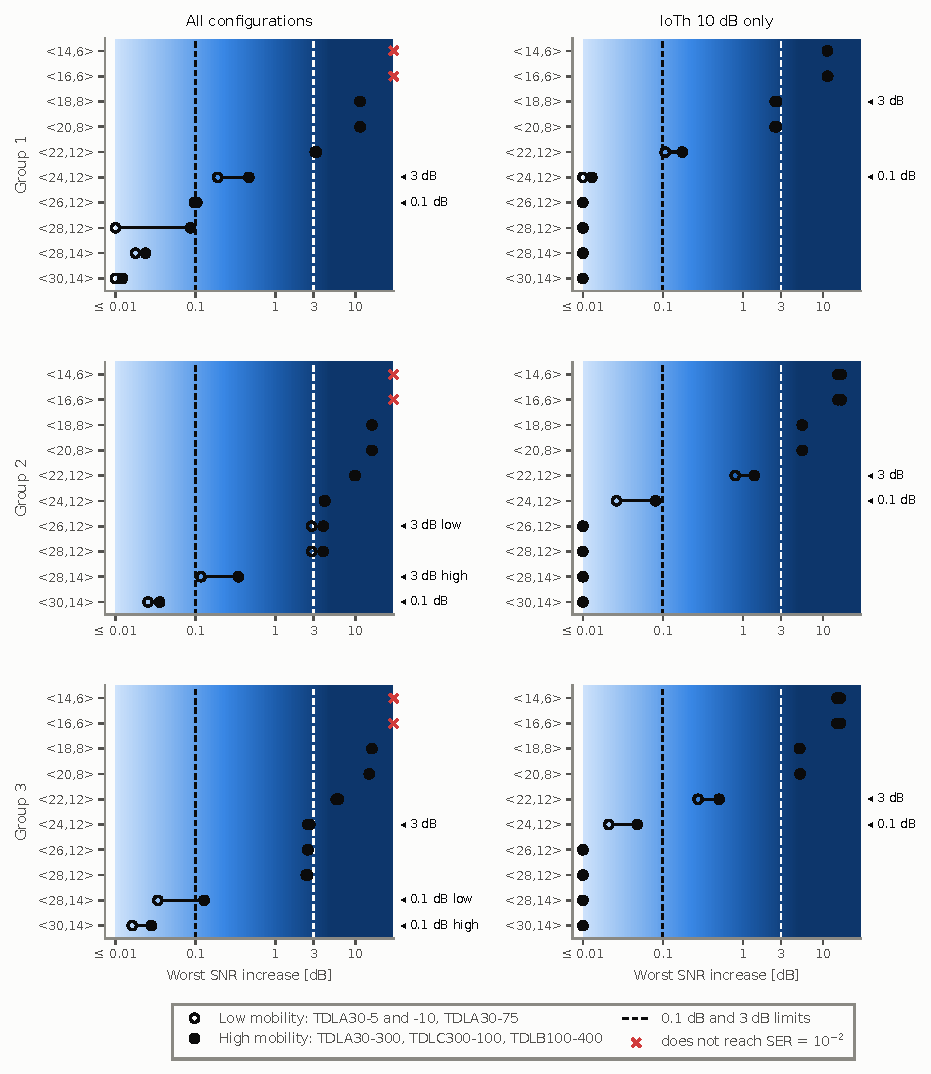
\includegraphics[width=\textwidth]{Images/RESULTADOS/perfis_mobilidade_formatos.pdf}
\vspace{4pt}
\legend{\textcolor{red}{Source: the author. Each format uses the same mode as in the SNR increase maps (Figures~\ref{fig:mapa-grupo1} to \ref{fig:mapa-grupo3}): RND\_ZERO/WRAP, except $\langle 14,6\rangle$ in RND\_MIN\_INF/SAT in group 1 and RND\_MIN\_INF/WRAP in groups 2 and 3; $\langle 16,6\rangle$ in TRN/SAT in group 1 and RND\_MIN\_INF/WRAP in groups 2 and 3; $\langle 18,8\rangle$ in TRN/SAT in group 3; and $\langle 30,14\rangle$ in TRN/SAT in all three groups.}}
\end{figure}


\FloatBarrier
% =====================================================================
\section{\texorpdfstring{SER curves}{SER curves}}\label{sec:resultados-curvas}\label{subsec:curvas-ser}
% =====================================================================

Figure~\ref{fig:curvas-ser-grupos} shows the SER curves for LMMSE and ZF (in floating-point) and BCD-MMSE (in fixed-point) for the TDLC300-100 channel model. The analysis here is not limited to the $\mathrm{SER} = 10^{-2}$ point; the curves cover the entire SNR range, from $-20$ to 10~dB. Each row of plots represents a group of configurations, while each column corresponds to a criterion from Table~\ref{tab:formatos-escolhidos}; the BCD-MMSE in each plot utilizes the format selected for that specific case. The first two columns include all configurations, the first with the 3~dB format and the second with the 0.1~dB format. The third column contains only the configurations with an IoTh of 10~dB, using the 3~dB format selected for them. The ZF performance remains unchanged by the format and is included in the plots as a worst-case reference; for the sake of clarity, it is omitted from the third column. The curves for the remaining test conditions can be found in Appendix~\ref{ap:curvas-ser}.

\begin{figure}[!htb]
\caption{\textcolor{red}{Curvas de SER dos três grupos na TDLC300-100, nos formatos escolhidos.}}
\label{fig:curvas-ser-grupos}
\vspace{4pt} % a classe zera o espaço entre a caption e a figura
\centering
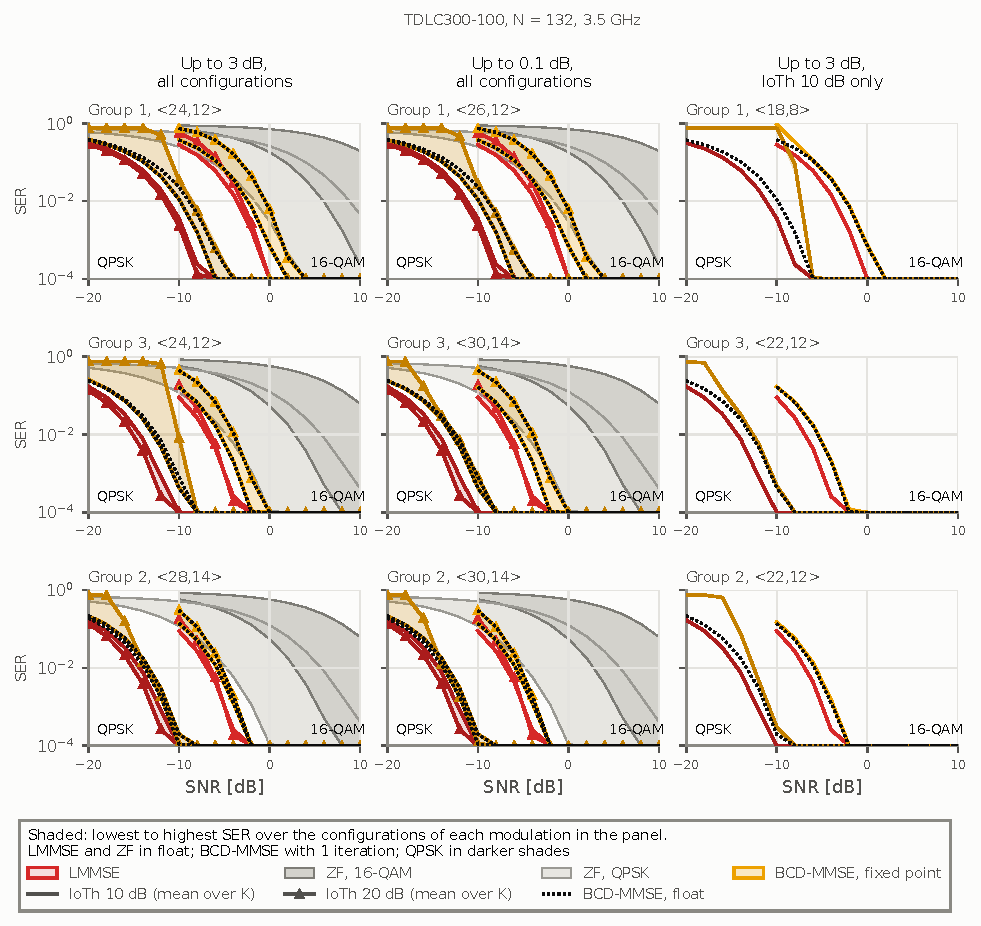
\includegraphics[width=\textwidth]{Images/RESULTADOS/curvas_ser/curvas_ser_grupos_range_C300.pdf}
\vspace{4pt}
\legend{\textcolor{red}{Fonte: a autora.}}
\end{figure}

Within a group, the configurations vary only in terms of soft constraints: modulation, $K$, and IoTh (Section~\ref{subsec:configuracoes-bs}). In each plot, the QPSK curves appear on the left in darker shades, while the 16-QAM curves appear on the right in lighter shades. The dotted line represents the floating-point BCD-MMSE, which serves as the reference for the format. Each curve represents the average between $K=8$ and $K=12$; these values differ by at most 0.9~dB at an SER of $10^{-2}$. The shaded region surrounding the curves spans from the lowest to the highest SER observed across the configurations of that modulation. Since $K$ has little impact, the width of this region in the first two columns primarily reflects the difference between IoTh values of 10~dB and 20~dB.

In floating-point arithmetic, QPSK operates at lower SNRs than 16-QAM (Section~\ref{subsec:simbolos}). In fixed-point arithmetic, however, some QPSK curves begin with a plateau: a flat, horizontal segment at the top of the plot, corresponding to an SER of 0.75. An SER of 0.75 implies that 3 out of every 4 symbols are incorrect, equivalent to a random selection among the 4 constellation points. Within this plateau, increasing the SNR does not improve the SER; beyond it, the curve drops sharply.

With a greater number of integer bits, the plateau ends at a lower SNR. In groups 1 and 2, the 0.1~dB format differs from the 3~dB format only by having more fractional bits, and the plateau ends at the same SNR. In group 3, the $\langle 30,14\rangle$ format has two more integer bits than the $\langle 24,12\rangle$ format, causing the plateau to end earlier. 16-QAM, on the other hand, operates at higher SNRs and shows almost no variation across the different formats. The exception is the $\langle 18,8\rangle$ format, where the 16-QAM curve begins above the floating-point curve, near $\mathrm{SER} = 1$, and quickly converges with it.

It should be noted that the LMMSE in the graphs is in floating point. Consequently, one cannot draw conclusions regarding how its performance varies with different IoTh values compared to the BCD-MMSE approach. It is observable, however, that the groups with smaller clusters (groups 1 and 3) exhibit the greatest gap between the BCD-MMSE curves for IoTh values of 10~dB and 20~dB, particularly when using 16-QAM (Figures~\ref{fig:descentralizacao-grupo1} and \ref{fig:descentralizacao-grupo3}).

Considering only the configurations with an IoTh of 10~dB, the 3~dB formats feature 2 to 6 fewer bits (Table~\ref{tab:formatos-escolhidos}). As shown in the third column, these formats remain within the 3~dB increase threshold at an $\mathrm{SER}$ of $10^{-2}$. Regarding the SNR increase of BCD-MMSE over LMMSE, no specific target was defined; nevertheless, this increase exceeds 3~dB only in the case of QPSK. This occurs in the smaller formats, $\langle 18,8\rangle$ for group 1 and $\langle 24,12\rangle$ for group 3, and, marginally, for the 1H configuration in $\langle 26,12\rangle$ (Figures~\ref{fig:descentralizacao-grupo1} and \ref{fig:descentralizacao-grupo3}). 

QPSK is the modulation scheme most sensitive to the number of bits because it operates at lower SNRs, where the elements of $\mathbf G_c$ are larger (Section~\ref{subsec:resultados-grupo2}). When these elements exceed the capacity of the chosen format, an integer overflow occurs, which results in a plateau (Section~\ref{subsubsec:ponto-fixo}). For instance, the $\langle 18,8\rangle$ format can store values up to 128. In the 1C case, the median of the largest element in $\mathbf G_c$ ranges from 70 at $-6$~dB to 164 at $-10$~dB. It exceeds the limit for nearly all matrices at $-10$~dB, while it does not exceed the limit for any matrix at $-6$~dB. It is within this range that the QPSK curve emerges from the plateau. Although the modulation scheme itself does not alter $\mathbf G_c$ (Section~\ref{subsec:hw-matrizes}), 16-QAM operates at higher SNRs, where such overflows occur less frequently.
